\documentclass{article}
\usepackage[utf8]{inputenc}
\usepackage{amsmath}
\usepackage{amssymb}
\usepackage{graphicx}
\usepackage{hyperref}

\title{Problem Solving Strategies - Chapter 2}
\author{Thomas Kidane}
\date{\today}

\begin{document}

\maketitle

\tableofcontents

\section{Introduction}
I have learned that solving all the problems in one section at a 
time are not good use of my time since I only learn to get better in 
competitive mathematics. So from now on I will do half the problems in 
each chapter and review it again after the end.

\section{Problems}

\subsection{Problem 1}

A rectangular floor is covered by $2 \times 2$ and $1 \times 4$ tiles. One tile got smashed. There is a tile of the other kind available. Show that the floor cannot be covered by rearranging the tiles.

\textbf{Solution}

I just need to make a coloring so that the colors in the $1 \times 4$ is diifferent from the colors in the $2\times 2$. Assume the rectangle 
in rows, where all the colors in a row are the same. And there four types of colors. The composiiton of the tiles of the tiles is different.

If you tried to change this by rearranging, then every ties will take up the same number of tiles?
Actually what if I just have two colors, colored row by row. Then how ever you arrange it, all the tiles will take up the same number of tiles 
from different colors? Is this even a valid example?

Ok after seeing the first solution I can use some of my knowledge from other sections as well(duh).

\begin{figure}[h!]
    \centering
    
\includegraphics[width=0.8\textwidth]{pic2.png}
    \caption{Descriptive caption of the image}
    \label{fig:example_image}
\end{figure}

\subsection{Problem 2}

Is it possible to form a rectangle with the five tetrominoes in Fig. 2.1?

\begin{figure}[h!]
    \centering
    
\includegraphics[width=0.8\textwidth]{pic3.png}
    \label{fig:example_image}
\end{figure}

If you color the grid with 2 colors(diagonally), the T terrino will always 
ahve either 2 black or 2 white extra cells. But the other have equal values and 
this is a contradiction since the rectanle must have equal number of both.

\subsection{Problem 3}

A 10 ×10 chessboard cannot be covered by 25 T-tetrominoes in Fig. 2.1. These
tiles are called from left to right: straight tetromino, T-tetromino, square tetromino,
L-tetromino, and skew tetromino.

\textbf{Solution}

Each T tetrino will either have extra 2 white or black cells. Since there 
are 25 of them, they can't cancel out. Does the sum need to be divisible by 
4? I don't know why I can't phrase this argument this way, even though it is
true? How can I turn it to a statement of 2 divisibility(even or odd).

The net sum of the exras should be 0. If I have 25 equal items and I can subtract 
them from each other, I can't get 0. Does it matter what the underlying stuff is?
No it doesn't, this statement is a case about divisibility. Can I describe it more eloquently?

No they come in pairs, so count the individual items in pairs too, so that 2 becomes 
1.

\subsection{Problem 4}

An 8$\times$8 chessboard cannot be covered by 15 T-tetrominoes and one square tetromino.

\textbf{Solution}

Same argument? The square will destory itself. I still get the same problem with odd number.

The books proof says that since for 60, half black and half white, you would need equal 
number of both types of tetrinoes. Better I guess.

\subsection{Problem 5}

A 10$\times$10 board cannot be covered by 25 straight tetrominoes (Fig. 2.1).

\textbf{Solution}

This requires some thinking. The normal checkerboard coloring isn't telling me anything.
Should I make a custom one for this problem? what characterisitic makes it 
impossible for the $4\times4$ to not be able to cover it?

I guess I need something that partially covers the tetrinoes?

What are the orientations? Can I make something that is equal for both orientations?

The tetrino always hits something that appears every 4 units? Does it?

Can I make it so that a tetrino doens't hit something more than once? That is 
not the same as hitting 4? I could make it so that it does?

How many of these 4 things can I place? I guess is 25? Can I place more?
If I can place more than 25 of these things but each tetrinbo can only hit 1 of
them, then I would be done? 10 mod 4 is 2? I can fit 3 in one row? all spaced 3 units 
apart. I shift this over one unit to the right on the next row. Since 4 doesn't 
divide 10 perfectly one of them will not align but that doesn't matter. 

How far is the distance vertically? There are a minimum of 3 units apart too.
In this fashion I have fit in 30 of these marked cells but each tetrino can only 
hit 1 of them. So it is impossible to tile the $10\times 10$ grid.

Would I have come up with these argument if this wasn't in this textbook? Probably 
not, I have been prompted, but I will not have this in a contest. I guess this is what
he was saying when he said that in an actual contest you don't know what type problem it will 
be, and I will only learn this skill doing a lot of probelms. Next problem.

Actually after reading the book, it had the same construction but 
instead it renamed each square with a number diagonally. It 
said that there 26 1's but no matter how you place it, there is only 1 that is 
being intersected, same I guess.

\pagebreak

\subsection{Problem 6}

Consider an $n\times n$ chessboard with the four corners removed. For which values of n
can you cover the board with L-tetrominoes as in Fig. 2.2?

\begin{figure}[h!]
    \centering
    
\includegraphics[width=0.8\textwidth]{pic4.png}
    \label{fig:example_image}
\end{figure}

\textbf{Solution}

Can I get a sufficient condition and worry about the necessary condition later?

Ok when is it suffient? I need a constrution(Oh constructive mathematics)?

Like in the picture I can $4\times 2$ blocks. Can I just extend the construction 
already in the picture? Lowkey I am going to do this tomorrow, it is 4:03 pm, But I shouldn't have 
been away from this for so long.

Ok I how do I extend the construction? I obviously can't make $n$s since I 
need an even amount of sqaures.I can't techinically do $2\times 2$ if you Consider
nothing as a sqaure. Can I make a $4\times 4$? Unfortunately impossible, why? 
Maybe I can extract a proof out of this?

Ok After reading the book it had a clean coloring. 

\begin{figure}[h!]
    \centering
    
\includegraphics[width=0.3\textwidth]{pic5.png}
    \label{fig:example_image}
\end{figure}

First of alll $n$ has to be even but you can look at the placement of the L tetrinoes
on the bottom board. It easier covers 3 balck or vice versa. Since are an equal number of
white and black cells. So are needs to be an equal number of tetrinoes. So the number of 
cells is divisble by 8. So $n^2-4 mod 8==0 \rightarrow n^2 mod 8==4$. This implies that 
$n mod 4 == 2$. Is this true? yes, I manually checked. But this also a form of divisibility 
but the problem is 4 and 8 shared a gcd so you have to divide the movule number  

\subsection{Problem 7}

Is there a way to pack 250 1 ×1 ×4 bricks into a 10 ×10 ×10 box?

\textbf{Solution}

I saw a variant of this problem in Math 283S. How do I do it? What if I have kind of like a checkerboard batter. 
Because this is reminisient of the $1\times2$ case on the $8\times 8$. 

I got the solution, first look at a $10\times 10$, grid, you can't fit in all
all the $1\times1\times4$ blocks on it. Because if you split the grid into 2 x 2 checkbaord 
board pattern, each $1\times 4$ block will hit 2, white and 2 black cells. That implies there 
would have to be an equal number of black and white cells but in this construciton there are an 
odd number of one of colors and therefore it is impossible.

So the trick when using pairty is that you try to modify the object you are using to prove that 
inequality, until you can make it odd and then you also make sure that your object hits it and 
even number of times. Just like invaraince.

Coming back to the cube, do the same thing but now with cubes of side lenth, any block will hit equal colors,
which implies equal colors of both, but that can't happen because are only 125 cubes. Therefore the construction is impossible.

The authors solutions is a bit similar and different. He first striped the cubes in 4 numbers, wherethe 
number of a certain cube is $(x,y,z) \rightarrow i mod 4$. For any layer of the 
cube, there are not going to be equal numbers of blocks, more specifically. Because $100 mod 4==2$.


Assign coordinates $(x, y, z)$ to the cells of the box, $1 \leq x, y, z \leq 10$. Color the
cells in four colors denoted by $0, 1, 2, 3$. The cell $(x, y, z)$ is assigned color $i$ if
$x + y + z \equiv i \mod 4$. This coloring has the property that a $1 \times 1 \times 4$ brick always
occupies one cell of each color no matter how it is placed in the box. Thus, if the box
could be filled with two hundred fifty $1 \times 1 \times 4$ bricks, there would have to be $250$
cells of each of the colors $0, 1, 2, 3$, respectively. Let us see if this necessary packing
condition is satisfied. Fig. 2.10 shows the lowest level of cells with the corresponding
coloring. There are $26, 25, 24, 25$ cells with color $0, 1, 2, 3$ respectively. The coloring
of the next layer is obtained from that of the preceding layer by adding $1 \mod 4$.
Thus the second layer has $26, 25, 24, 25$ cells with colors $1, 2, 3, 0$, respectively. The
third layer has $26, 25, 24, 25$ cells with colors $2, 3, 0, 1$, respectively, the fourth layer
has $26, 25, 24, 25$ cells with colors $3, 0, 1, 2$, respectively, and so on. Thus there are
$(26 + 25 + 24 + 25) \cdot 2 + 26 + 25 + 251$ cells of color $0$. Hence there is no packing.

\subsection{Problem 8}

An $a \times b$ rectangle can be covered by $1 \times n$ rectangles iff n$\vert$a or n$\vert$b.

\textbf{Solution}

Now I am proving the general theorem interesting. Assume that that n doesn't divide both 
$a$ and $b$.

Number each $(x,y) \rightarrow (x+y) mod n$, on the first row there are $a mod n$, extra numbers, of some kind.
One row below is just the same extras shifted one unit over, doing this b times you $b mod n$, extra times.

All of this squares can't be equal because each number doesn't have an equal amount, let me try to do an 
algebraic equation or argument. Imagine you have n zeros $0,0,...,0$ these represent how much extra 
each number has. The operation we do each time is basically add a continious string of 1 of lenght $a mod n$.

If we do these process n times we can start from 0, again. So the result is the same as doing this process $b mod n$ times.

After seeing the authors solution I will edit it. Make each row a single number. 
$a=qn+r$, where r is greater than 0 and less than. You will have $qb+b$ colors of $1,...,r$ and $qb$ colors of the 
rest. Every time you place an $1\times n$ block you either cover all colors equally or n times of a single color.

Let's say you place all the $h$ blocks so the number of colors are now $bq+b-h$ and $bq-h$. 
That means each column is now divisible by $n$. But that also implies that n also divides their difference 
therefore $n\vert b$. Which is nonsense. Same proof works in the case of 3d space.

\subsection{Problem 9}

One corner of a $(2n + 1) \times (2n + 1)$ chessboard is cut off. For which $n$ can you
cover the remaining squares by $2 \times 1$ dominoes, so that half of the dominoes are
horizontal?

\textbf{Solution}

How many domnioes are there? $(2n+1)*(2n+1)-1=4n^2+4n \rightarrow 2n^2+2n$ dominoes 
that are tiled horizontally. That also means there are the same number vertically as well.

Can I do this for 1x1, yes, 2x2, no. It has to be odd first.
So 3x3? No I can't 
5x5? yes.

Is it flip flopping? So n has to be of the form even?

I kind of want to make an operation that treats horizontal and vertical blocsk differently.
How do I do that? 

Can I somehow use the fact that there are an equal number of vertical and horizontal blocks?


Actually $4\vert 4n^2+4n$. Which gives me nothing much. What is wrong with n begin odd?
Why can't I do it for $2\times 2$?

Ok I have the proof for even numbered sides. First if the side of the square is
$n\times n$, color it so that there is only one color on each row, and it is in alternating fashion.

Now each vertical block decreases the total number of black and white by 1 each. 
The other one decreases a single one by 2. What can you do is that you can place all the 
vertical ones first, so if there are $n^2/2$ colors of each side, you do a quarter of those opertions first?

There are $n^2$ cells. I can do $n^2/2$ opertions. Out of these half will decrease both by one
so the total number of both opertions after doing all the veritcal operations is 
$n^2/2 - n^2/4$. And after this all opertations decrease this number by two so, it has to be divisible by 2.

So we get $2\vert n^2/2-n^2/4 \rightarrow  2\vert n^2/4 \rightarrow 8\vert n^2$. But since this is square,
there are an even power of 2s, therefore $n$ must atleast be divisible by 4.

Lets go back to our problem, there are $4n^2+4n$ total colors. Out of these $2n^2+2n$ colors are of one specific color.
I can decrease this by half and this has to be divisible by 2 too. So $2\vert n^2+n$. 

When is this satisfied? Always? I have the answer for even vales, how I can extend this to the odd values.
I can fill out the sides with equal number of whites and blacks and I can show 
the problem doesn't work.

Oh fuck, after looking at the first senstence of the author's solution, I realized 
that my assumption that there were an equal number of number of white and black cells was wrong. 
There are actually $(2n+1)*(n)$ of one color and $(2n+1)*(n)+2n$ colors of  the other.

This translates into $2n^2+n$ and $2n^2+3n$ colors. Same idea as before, I can decrease both, by
$n^2+n$ and get that $2\vert n^2$ and $2\vert n^2+2n$. This leads us to say $2\vert n$. I just wish I 
had more attention into the actuall numbers of elements. The idea of taking differences, was there.

I actually also have to prove that this is suffient. So assuming that n is even,
I have to make some construction to fulfill. First just fill the ones on the top and right with ones of their corresponding side. 
This has equal number of both. Then the inner square is $2n\times 2n$. Which is simple since you can make $2n\times n$ one side and do this for both 
of the block types.

\subsection{Problem 10}

Fig. 2.3 shows five heavy boxes which can be displaced only by rolling them about
one of their edges. Their tops are labeled by the letter $\top$. Fig. 2.4 shows the same
five boxes rolled into a new position. Which box in this row was originally at the
center of the cross?


\textbf{Solution}

I actually wasted a lot on this problem, because I was trying to move the squares 
to the positions required.

Doesn't matter now, so basically the authors answer is that if you make a checkerboard 
patter on the the board, you will that there is one color with 4 T's and 1 colors 
with one T.

Now to go from T to T requries and even number of moves. Since 1,3,4,5 are on T.
They are also on the color they started with. Since 1,3, and 5 are on the same color,
they must be on the color that had 4, units. Since the Rotated 90 degree T shapre
requires and odd number of moves, the 2nd one is the color that it doesn't belong to.
There fore it was also in the one with 4 cubes, therefore the central element is the 4th one.

\subsection{Problem 11}

Fig. 2.5 shows a road map connecting 14 cities. Is there a path passing through each
city exactly once?

\textbf{Solution}

I think this is graph theory question, about hamiltonian path?

Since I can only visit each city once, that also means I can only gone along 
an edge once. There are 8 cities with 3 edges each, and 6 cities with 4 edges each.

Let say the path starts at a node that has 4 edges, Then it must start and end at that point.
And the cities with 4 edges will just be cities that connect i

Actually that logic is flawed, this isn't an eulerian path.

It is a bipartite graph. Could I do something with the path length?

After looking at the solution I realized that I forget to account for the 
fact that there weren't an equal number of black and white cells. Since it is 
bartitie and it flip flops, there must be an equal number, of each color. Oh stupid me.

\subsection{Problem 12}

A beetle sits on each square of a $9 \times 9$     chessboard. At a signal each beetle crawls
diagonally onto a neighboring square. Then it may happen that several beetles will
sit on some squares and none on others. Find the minimal possible number of free
squares.

\textbf{Solution}

What is maximum amount the ants could compressed in? Actually since ants 
move diagonally the mod 2 sum of their coordinates never changes. Since it 
started off at 2, is can't get any lower than that.

I need a construction for the other side. All ants will go to one side, then they will move 
to one diagonal, then they will converge. Then we are done.

OK after I read the solution, it was wrong. I should be answering the question 
of what is the minimum number of spots that are not occupied. 

The solution is that if you color the columns alternatingly, white and black. 
There are 45 and 36 colors of each, and each move changes the colors of the beetles.
Therefore atleast 9 stay free? I guess that makes sense.


\subsection{Problem 13}

Every point of the plane is colored red or blue. Show that there exists a rectangle
with vertices of the same color. Generalize.

\textbf{Solution}

Ok so I tried and argument where I constantly look to the left or to thr right and
try to extend corners until I got a recetangle but, tghe authors solution is very simple 
and it works for mulitple colors. Assume you have $n$ colors instead of 2 colors. 

Then take the latice points $(x,y)$ where the componenets are integers and 
$1 \leq x \leq n+1$ and $1 \leq y \leq n^{n+1}+1$. The number of ways to color 
a row of n+1 elements is $n^{n+1}$ and due to the pigeonhole principle 
there must atleast be atleast one repeated color. Since we list out more 
more than all the combinations of colors possible, there must atleast 
be one combination that is listed out twice. So we can make a rectanle out 
of this since there are 4 colors and they all have right angles between them.

I think we can generalize this to higher dimensions? Like into 3d, and 
have cubiods, and maybe 4 dimensions? I think so.

\subsection{Problem 14}

Every space point is colored either red or blue. Show that among the squares with
side 1 in this space there is at least one with three red vertices or at least one with
four blue vertices.

\textbf{Solution}

I guess I can swap this statement since the exact colors don't matter. 
So there is one with all red or one with 3 blue vertices and vice versa.

I just have to show that athere can't be all 2 of each. So not 
everything is 2 red and 2 blue. Let's say I am stating on a blue point.
Then one unit forward is another red point. Then at a right angle to the 
right and left, there are 2 other points. They could be one of four combinations.

I will think about this tomorrow.
I actually looked at the answer and it was very complicated, I don't think 
there is any point in learning it.

\subsection{Problem 15}

Show that there is no curve which intersects every segment in Fig. 2.6 exactly once.

\begin{figure}[h!]
    \centering
    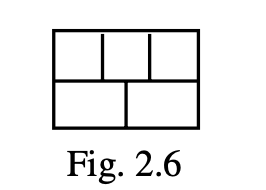
\includegraphics[width=0.3\textwidth]{pic6.png}
    \label{fig:example_image}
\end{figure}

\textbf{Solution}

What does segement mean? I hate when problem statements are not clear. Ok can I think of the segments as edges?

Ok after reading I understand that the the four boxes(one in top middle, 2 in the bottom and the out surface)
each have five segments, therefore the paths must start and end in the odd faces, but that can't be the case 
because a path either has no starting points or two.

\subsection{Problem 16}

On one square of a 5 ×5 chessboard, we write -1 and on the other 24 squares +1.
In one move, you may reverse the signs of one a ×a subsquare with a $>$ 1. My goal
is to reach +1 on each square. On which squares should -1 be to reach the goal?

\textbf{Solution}

Ok from what I can think of, the 4x4 case doesn't matter.
Is there a spot I can put the -1, such that this will work? I think that it is
impossible? Maybe I need to prove that overlaying any number of susquares on the 
the $5\times 5$, that is valid will never have a single point that is covered an odd number

How should I color the grid then? Ah, I have images in my mind(why did I look at the solutions?).
Well I don't know if it works but let me to try derive it fromn first priniples.

So what I want is somethign that stays conserved under the applying the subsquare forms.
For the even, I want to hit an even number of items. For the odd ones, I guess I also need an odd amount. 

Since I have thie 5 case, that means the total in the square is odd. Then it also has to be 
the case that the $3\times 3$, is odd. If I nudge, a $3\times 3$ square a little bit,
then the inner $2\times 2$ is conseved, but the outer ones change. I know that there are an 
even number in the conversed $2\times 2$ case, so in the out 5 places, there were an odd number.

Infact because I can push it in every direction, there is a odd in the outer layer from every 
perspective. There can be either 1, 3, or 5? Since it is odd in every direction?

I also need it to be translation invariant. So every strip of 5 L, should have an odd number. I guess checkerboard,
but it is only invarinat under a diagonal move, when I nudge the square to the side horizontally, the 
parity of the number changes. When I do a tranlation whether vertically or horizontally, I am losing 
3 blocks and replacing them with another 1, and 2. So these have the same parity.

So every 3 spots it is the same? and same with a $1\times 2$ move sideways? I think I have an idea.

Color the board like these: first row becomes, all zeros. Second row becoems alternating 1 and 2, repeat process.

If I do a move of $2\times 2$, then it has no effect on the mod 3, sum of the entire baord.
If I do a move of $5\times 5$? If 3 rows are zero, then no change happens. Since there are an 
equal number of 1s and 2s. What happens in the case of $3\times 3$? Fucked!

Well I couldn't my insight of the $3\times 3$ case into an actual solution.

Here is the stated solution.

\begin{figure}[h!]
    \centering
    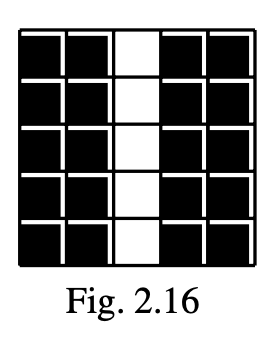
\includegraphics[width=0.3\textwidth]{pic7.png}
    \label{fig:example_image}
\end{figure}

Every permitted squares an even number of black squares. If the -1, is on 
the black squares you are cooked and by 90 rotation the only thing left is the center.

You can get the center by first doing the lower left corner $3\times 3$, then the upper right 3, then lower right and upper left 2.
Then the whole thing.

\subsection{Problem 17}

The points of a plane are colored red or blue. Then one of the two colors contains
points with any distance.

\textbf{Solution}

Lowk this is cooked but, let me see if I can do it? Since the distance is continious, I 
might have change my approach. Assume the red color doesn't have every every distance, 
then that means for every red point, the circle around of some radius is made of entirely blue stuff. Then 
there are either finitely many red points or infinetly many? But either the circles are intersecting 
or there are points that fill the distance in between them so you can make a radius of any distance you want?

This is not really rigrours. Let me try again.


If both colors have all distances reachable then there is nothing to prove. Assume that color A has a distance isn't 
reachable to it, therefore every point with color has A has a circle around of it with the unreachable distance. This implies 
that all the distances are reachable from color B, assume for the sake of contradiction that there is some distance 
that is also not reachable from B. But that would imply that this distance is reachable from and A and all the distances less than it,
contradicting the assumpiton that the previous distance wasn't reachable from A.

\subsection{Problem 18}

The points of a plane are colored with three colors. Show that there exist two points
with distance 1 both having the same color.

\textbf{Solution}

I will only consider the lattice points. Can I prove that there atleast has 
two be two points with the same color that share an edge?



Lowk I think I have had enoug of this chapter for now. Onto the next!



\end{document}

